% !TeX root = main.tex

% ============================================================
% thesis-sync entry: 2026-07-06_fabrication-molding-process
% Type: design decision (process) 
% Insertable section block (no preamble). Requires: graphicx.
% Figure \includegraphics lines are COMMENTED so the file compiles standalone.
% ============================================================

\section{FABRICATION}
\label{sec:lizard-fabrication}

\subsection{Mold Design for the Three-Chambered Segment}

Casting a 6~mm diameter tube with three internal 120$^{\circ}$ chambers
and a 0.4~mm outer wall places tight tolerance demands on the mold. The
mold assembly consists of: (i) three 120$^{\circ}$ fan-shaped chamber
cores machined in brass, which form the internal chambers and define the
internal walls converging at the axis; (ii) an acrylic cover pair with a
semicylindrical cavity, which forms the outer surface of the tube; and
(iii) 0.5~mm acrylic spacer plates with a three-lobed cutout, which
register the brass cores concentrically inside the cavity at both ends. The spacers hold the three brass cores at the correct
angular spacing, and uncured EcoFlex 00-30 is
cast into the closed mold.

\subsection{Demolding by Capillary Release}

Extracting the three brass fan cores from the cured 0.4~mm-walled tube
without tearing the silicone proved to be a critical fabrication step.
The adopted solution exploits capillary action as a liquid mold release:
a tweezer tip wetted with ethanol is inserted between each brass core and
the cured silicone, and the ethanol is drawn along the core--silicone
interface by capillarity, acting as a temporary release agent over the
whole contact surface. The cores can then be withdrawn without damaging
the internal walls. The ethanol subsequently evaporates without residue.

\subsection{Fiber Application}

After demolding, the circumferential reinforcement is applied by dipping
the cast tube in uncured silicone and winding the fiber by hand as
discrete parallel loops; the excess silicone is removed by scraping each
fiber loop with tweezers. The resulting average loop spacing is 1.5~mm,
with the deviation from perfect regularity attributable to the manual
process. The central axial fiber is placed through the junction of the
three internal walls, and the longitudinal constraint fiber of the leg
actuators is placed along the tube side before the reinforcement coat
cures. The end caps, foot interfaces, and suction cups are cast
separately in Elastosil M4601 and bonded to the cured tubes as described
in Section~\ref{sec:lizard-materials}.

% --- Figures (paths to be fixed by the author; commented for compilation) ---
\begin{figure}[tb]
  \centering
  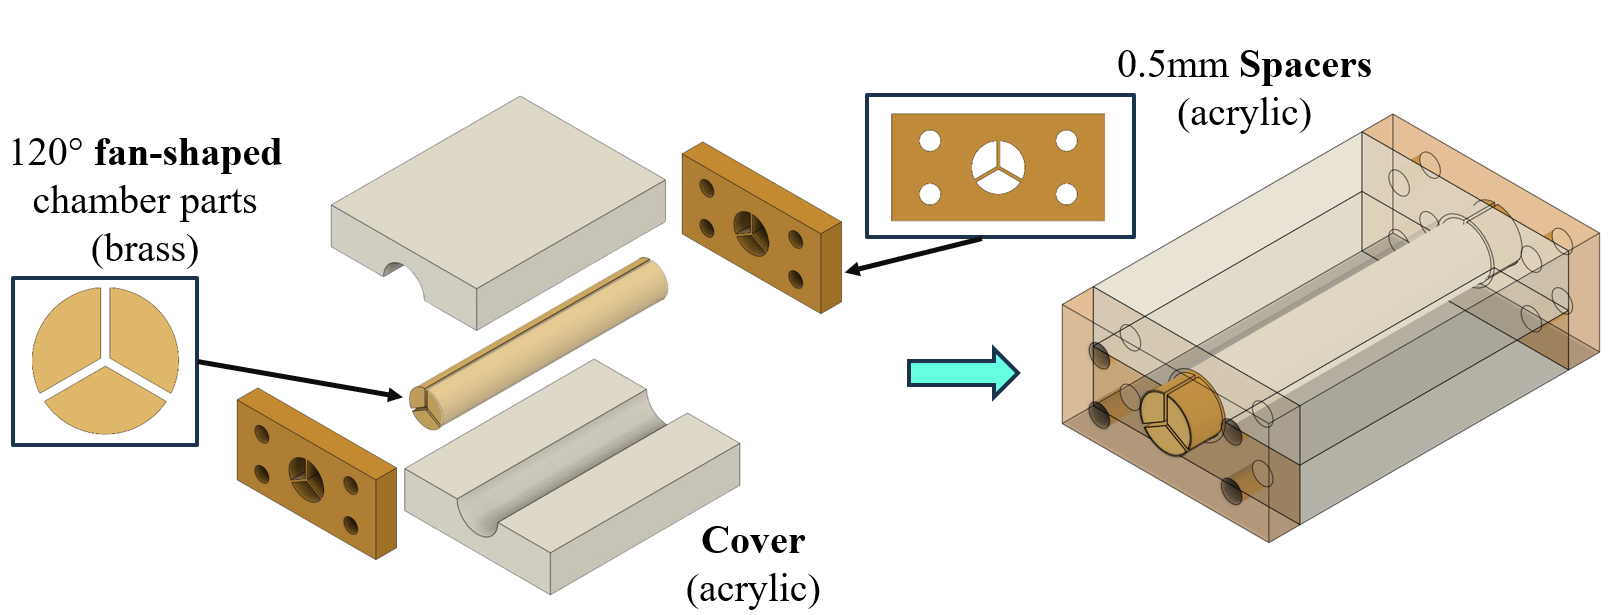
\includegraphics[width=0.95\columnwidth]{figures/threechambermold.png}
  \caption{Exploded and assembled views of the mold for the miniaturized
  three-chambered segment. (a)~The three 120$^{\circ}$ fan-shaped brass
  chamber cores. (b)~The 0.4~mm acrylic spacers that register the cores. (c)~The acrylic cover forming the
  outer surface of the 6~mm tube. (d)~The assembled mold.}
  \label{fig:lizard-mold}
\end{figure}
